%% Diagram to illustrate the algorithm
\documentclass[8pt, tikz]{standalone}

\usetikzlibrary{arrows.meta, bending, decorations.pathreplacing, positioning, shapes}

\tikzstyle{every picture}+=[remember picture]
\tikzset{
    neuron/.style = {
      fill=gray, circle, text width=5pt, text height=5pt, inner sep=0,
      draw=black!65!white, ultra thick,
    },
    box/.style = {
      ultra thick, color=black!70!white, draw,
    },
    ringbuffer/.style = {
      box, circle, text width=7.5pt, text height=7.5pt, inner sep=0,
    },
    matrix line/.style = {very thick, draw=black!50!white},
    relation/.style = {line width=2.5pt, black!45!white, arrows={Triangle[]-Triangle[]}},
    core/.style = {line width=4pt, draw=black!10!white, inner sep=10pt},
    link/.style = {ultra thick, black!80!white, arrows={-Triangle[]}, shorten >= 2pt},
    brace/.style = {decoration={brace, amplitude=5pt}, decorate, very thick},
    brace label/.style = {midway, align=center},
    brace label above/.style = {brace label, above=5pt},
    brace label below/.style = {brace label, below=5pt},
    value packet split/.style = {very thick, black!50!white},
    packet/.style = {above=2.5pt, text height=5pt, inner sep=0, value packet split, draw},
    spike packet/.style = {packet, text width=5pt},
    value packet/.style = {packet, text width=10pt},
}

\newcommand{\drawmatrix}[3]{%
  \draw [matrix line] (#1) rectangle ++(10pt * #2, -10pt * #3);
  \foreach \i in {2,...,#2}{%
    \draw [matrix line] ([xshift=10pt * \i - 10pt] #1) -- ++(0pt, -10pt * #3);
  }
  \foreach \j in {2,...,#3}{%
    \draw [matrix line] ([yshift=-10pt * \j + 10pt] #1) -- ++(10pt * #2, 0pt);
  }
}

\newcommand{\valuecore}[4]{%
  %% Draw a value-based transmission core:
  %% Arguments:
  %%    1. Name prefix
  %%    2. Number of neurons
  %%    3. Number of encoder dimensions
  %%    4. Number of decoder dimensions
  \begin{tikzpicture}
    %% Draw the filter and the encoder matrix
    \node [box, minimum width=40pt, minimum height=30pt]
         (#1_filter) {$H[z]$};
    \node [box, minimum height=#2*20pt + 5pt, minimum width=#3*10pt + 10pt,
           right=30pt of #1_filter.east] (#1_encoder) {
             \begin{tikzpicture}
               \drawmatrix{0pt, 0pt}{#3}{#2}
             \end{tikzpicture}
           };

    %% Connect them together
    \draw [link] (#1_filter) -- (#1_encoder);

    %% Draw the neurons
    \foreach \n in {1,...,#2}{%
      \node [right=25pt of #1_encoder.south east, neuron, yshift=\n*20pt - 7.5pt]
            (#1_\n) {};
      \draw [link] (#1_encoder.east |- #1_\n) -- (#1_\n);
    }

    % Draw the decoder
    \node [box, right=55pt of #1_encoder.east, minimum width=#4*10pt + 10pt,
           minimum height=#2*20pt + 5pt] (#1_decoder) {
            \begin{tikzpicture}
               \drawmatrix{0pt, 0pt}{#4}{#2}
            \end{tikzpicture}
           };

    %% Connect the neurons to the decoder
    \foreach \n in {1,...,#2}{%
      \draw [link] (#1_\n) -- (#1_\n -| #1_decoder.west);
    }
  \end{tikzpicture}
}

\newcommand{\spikescore}[3]{%
  %% Draw a value-based transmission core:
  %% Arguments:
  %%    1. Name prefix
  %%    2. Number of neurons
  %%    3. Number of pre-synaptic neurons
  \begin{tikzpicture}
    %% Draw the filter and the encoder matrix
    \node [box, minimum height=#2*20pt + 5pt, minimum width=#2*10pt + 10pt]
          (#1_weights) {
             \begin{tikzpicture}
               \drawmatrix{0pt, 0pt}{#2}{#3}
             \end{tikzpicture}
           };

    %% The multiplex which takes spikes and produces packets.
    \node [trapezium, box, rotate=-90,
           minimum width=20pt * #2, minimum height=15pt,
           trapezium stretches, trapezium angle=75,
           right=117.5pt of #1_weights.east, anchor=south] (#1_mux) {};

    %% Draw the ring buffers and the neurons
    \foreach \n in {1,...,#2}{%
      \node [right=30pt of #1_weights.south east, ringbuffer, yshift=\n*20pt - 7.5pt]
            (#1_ringbuffer_\n) {};
      \node [right=30pt of #1_ringbuffer_\n, neuron] (#1_\n) {};

      \draw [link] (#1_weights.east |- #1_ringbuffer_\n) -- (#1_ringbuffer_\n);
      \draw [link] (#1_ringbuffer_\n) -- (#1_\n);
      \draw [link] (#1_\n) -- (#1_\n -| #1_mux.south);

      \draw [box, very thick, arrows={-Straight Barb[bend, width=3pt, length=3pt]}]
        (#1_ringbuffer_\n.center)++(-45:10pt)
        arc [start angle=-45, delta angle=-90, x radius=10pt, y radius=10pt];
      \draw [box] (#1_ringbuffer_\n.north west) -- (#1_ringbuffer_\n.south east);
      \draw [box] (#1_ringbuffer_\n.south west) -- (#1_ringbuffer_\n.north east);
    }
  \end{tikzpicture}
}

\begin{document}
  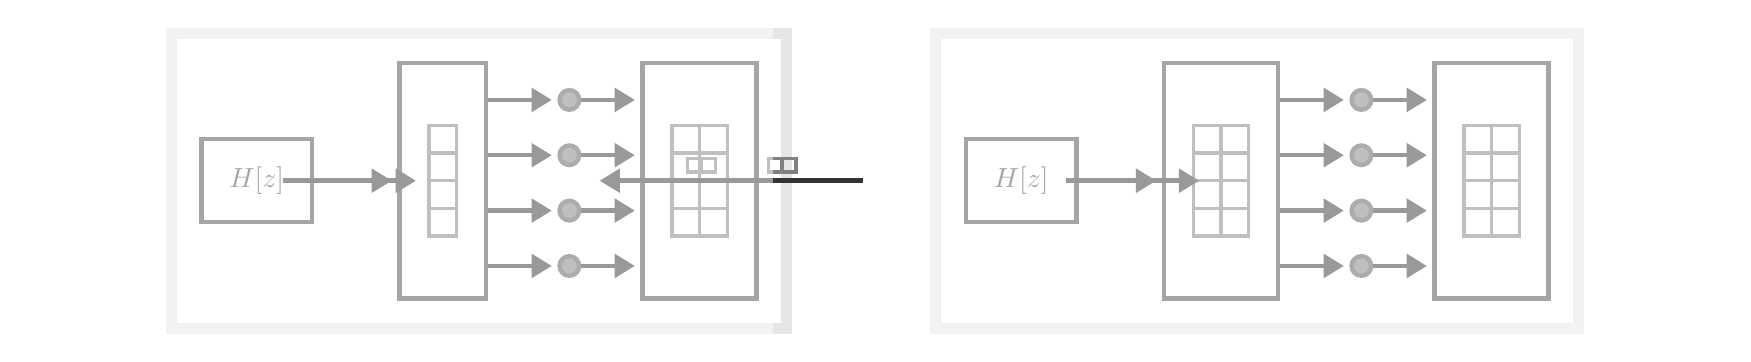
\begin{tikzpicture}
    %% Create the two cores and connect them
    \node [core] (A) {\valuecore{A}{4}{1}{2}};
    \node [core, right=50pt of A] (B) {\valuecore{B}{4}{2}{2}};
    \draw [link] (A_decoder) -- (B_filter)
      node [pos=.3, value packet] (val1) {}
      node [pos=.6, value packet] (val2) {};
    \foreach \n in {1,2}{%
      \draw [value packet split] (val\n.north) -- (val\n.south);
    }

    %% Draw extra input and output connections
    \draw [link] ([xshift=-50pt] A_filter.west) -- (A_filter.west);
    \draw [link] (B_decoder.east) -- ++(50pt, 0);

    %% Hide the earlier part of A and the latter part of B
    \fill [fill opacity=0.5, white]
    ([xshift=-2.5pt] A_4.west |- A.north west) rectangle ([xshift=-50pt] A.south west);
    \fill [fill opacity=0.5, white]
      (B_4.east |- B.north east) rectangle ([xshift=50pt] B.south east);
  \end{tikzpicture}

  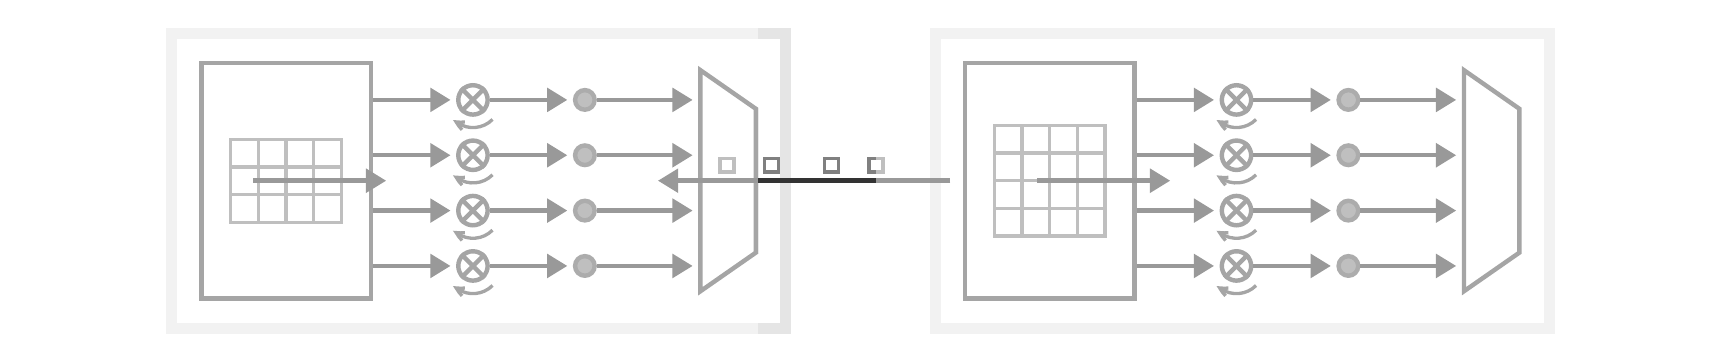
\begin{tikzpicture}
    %% Create the two cores and connect them, mark spike packets should be placed
    \node [core] (A) {\spikescore{A}{4}{3}};
    \node [core, right=50pt of A] (B) {\spikescore{B}{4}{4}};
    \draw [link] (A_mux.north) -- (B_weights)
      node [pos=0.25, spike packet] (sp1) {}
      node [pos=0.40, spike packet] (sp2) {}
      node [pos=0.60, spike packet] (sp3) {}
      node [pos=0.75, spike packet] (sp4) {};

    %% Draw extra input and output connections
    \draw [link] ([xshift=-50pt] A_weights.west) -- (A_weights.west);
    \draw [link] (B_mux.north) -- ++(50pt, 0);

    %% Hide the earlier part of A and the latter part of B
    \fill [fill opacity=0.5, white]
    ([xshift=-2.5pt] A_4.west |- A.north west) rectangle ([xshift=-50pt] A.south west);
    \fill [fill opacity=0.5, white]
      (B_4.east |- B.north east) rectangle ([xshift=50pt] B.south east);
  \end{tikzpicture}
\end{document}
